\chapter{Eksploratorna analiza}

\section{Opis atributa}
opis atributa....

\section{Proces učitavanja i prilagodbe podataka}

	\subsubsection{Proces učitavanja podataka}
	
	\textbf{Opis grafa:}
	
	Ovaj graf prikazuje histogram popularnosti. Prikazuje distribuciju popularnosti pjesama. Na x-osi nalaze se razine popularnosti pjesama, a y-osi broj pjesama koje se nalaze u pojedinoj razini popularnosti.
	Ovaj histogram omogućava vizualni pregled koje su razine popularnosti češće, a koje rjeđe. 
	
	\textbf{Slika grafa:}
	\begin{figure}[H]
		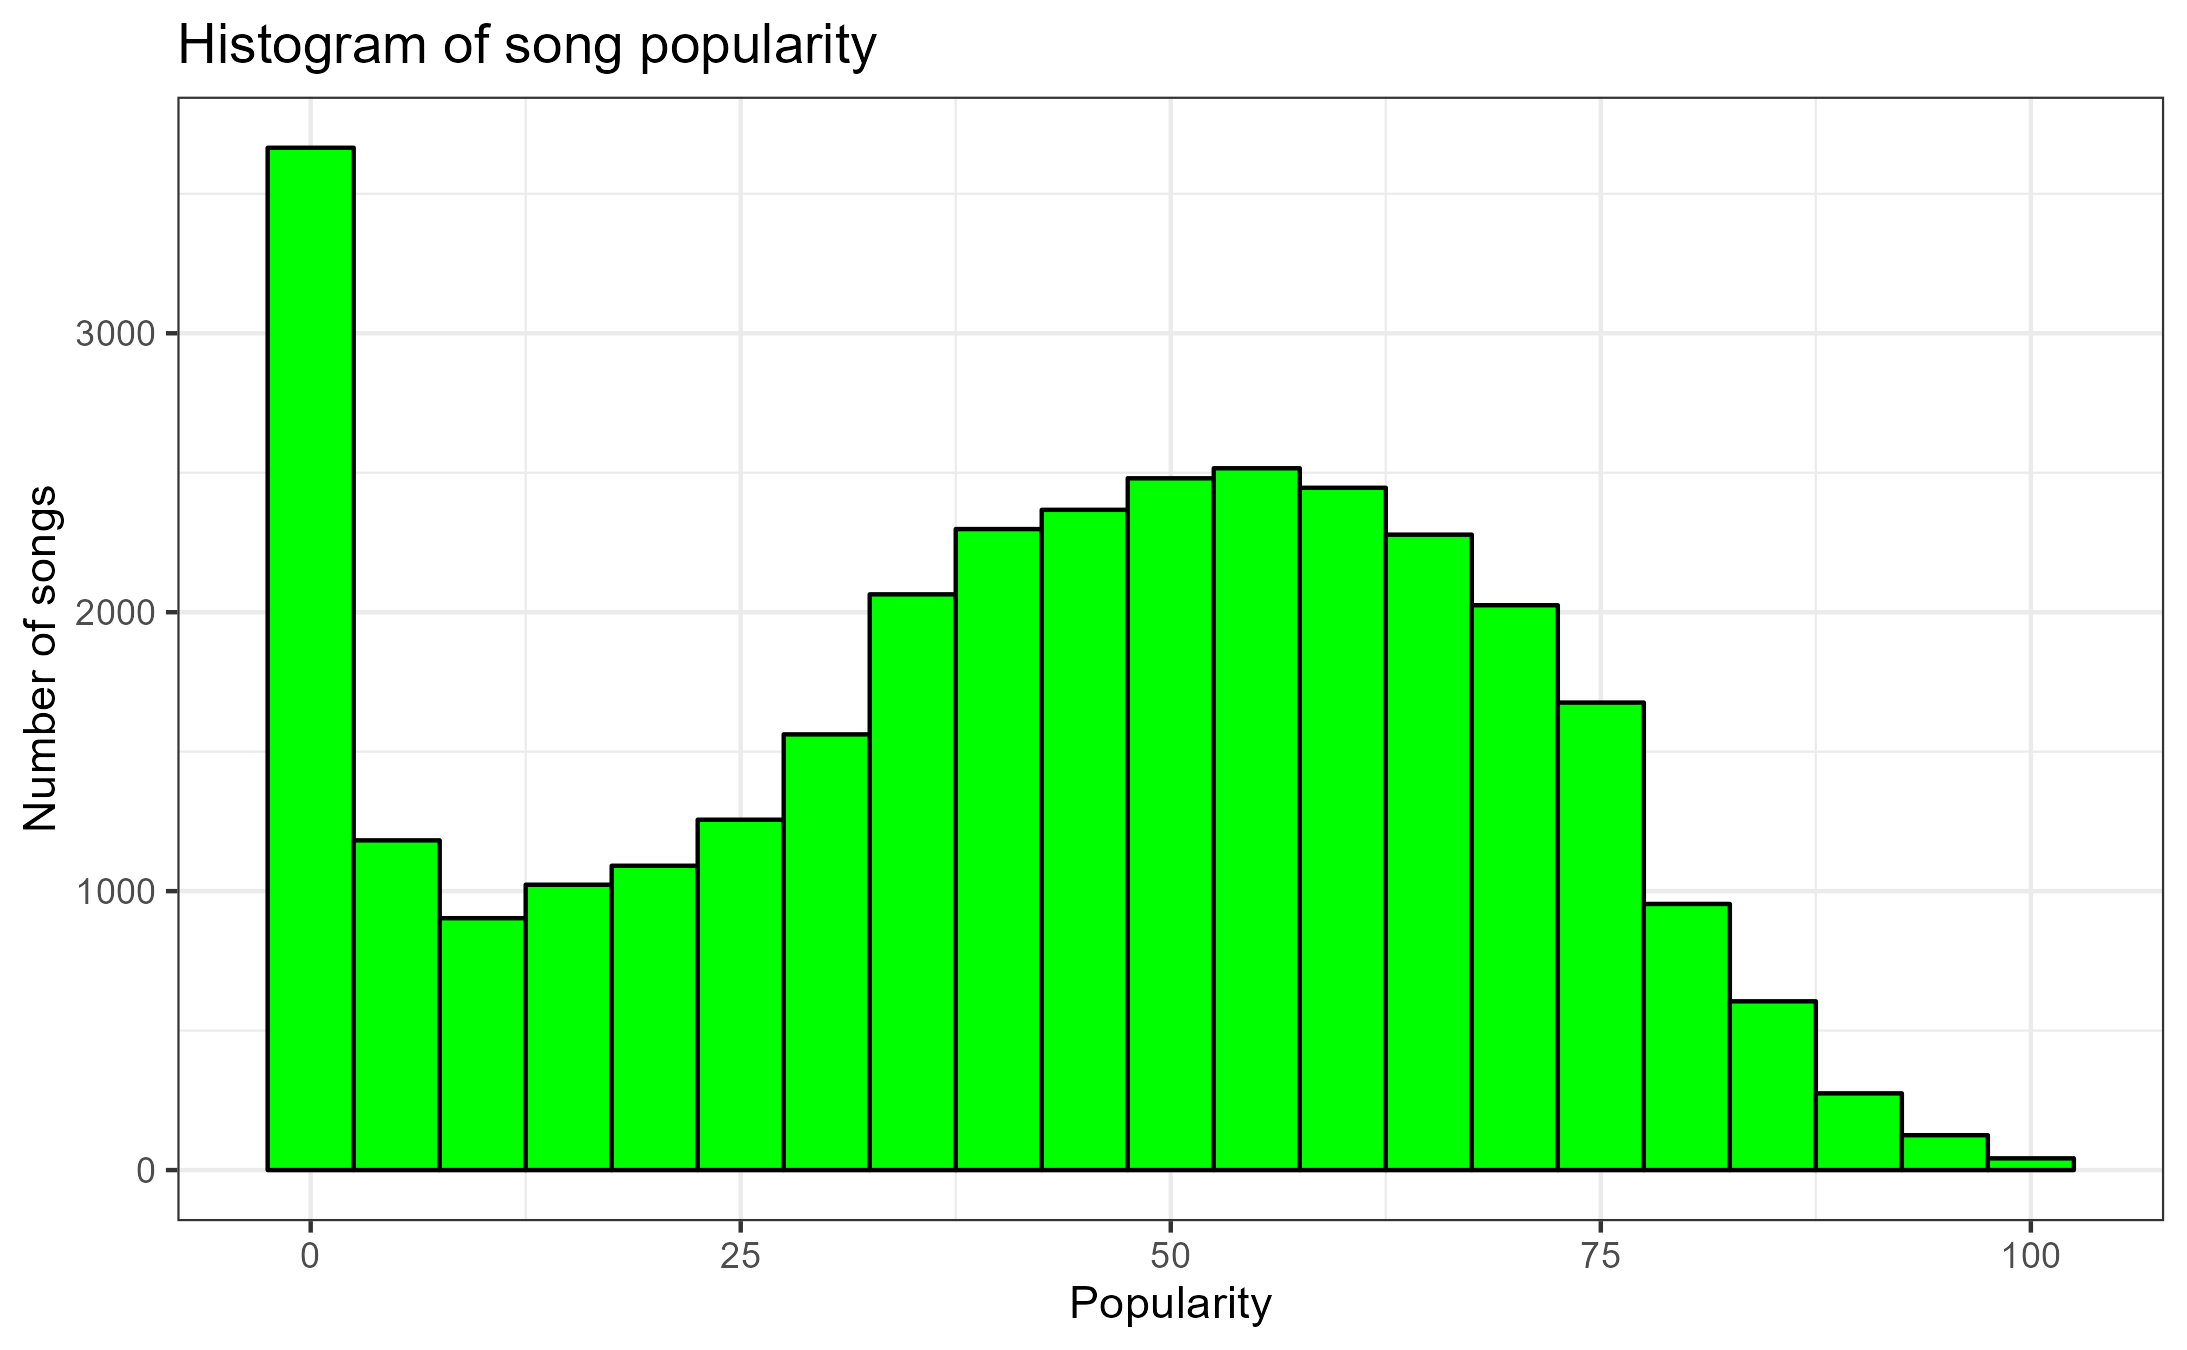
\includegraphics[scale=0.9]{slike/Histogram of song popularity.png}
		%veličina slike u odnosu na originalnu datoteku i pozicija slike
		\centering
		\caption{Histogram of song popularity}
		
	\end{figure}
	
	\subsubsection{Proces prilagodbe podataka}
	
	\textbf{Opis grafa:}
	
	Ovaj graf prikazuje deset najpopularnijih glazbenih izvođača temeljem prosječne popularnosti njihovih pjesama. Izračunata je srednja vrijednost popularnosti za svakog izvođača po njegovim pjesmama, a zatim su odabrani najbolji deset izvođača prema toj mjeri popularnosti.
	
	Na x-osi su navedeni izvođači, poredani prema visini prosječne popularnosti, dok y-os prikazuje prosječnu popularnost. Svaki šareni stupac predstavlja jednog izvođača, a visina stupa označava njegovu prosječnu popularnost.
	
	Ovaj graf pruža brz i pregledan način usporedbe popularnosti izvođača, omogućujući identifikaciju najboljih deset temeljem prosjeka popularnosti njihovih pjesama.
	
	\textbf{Slika grafa:}
	\begin{figure}[H]
		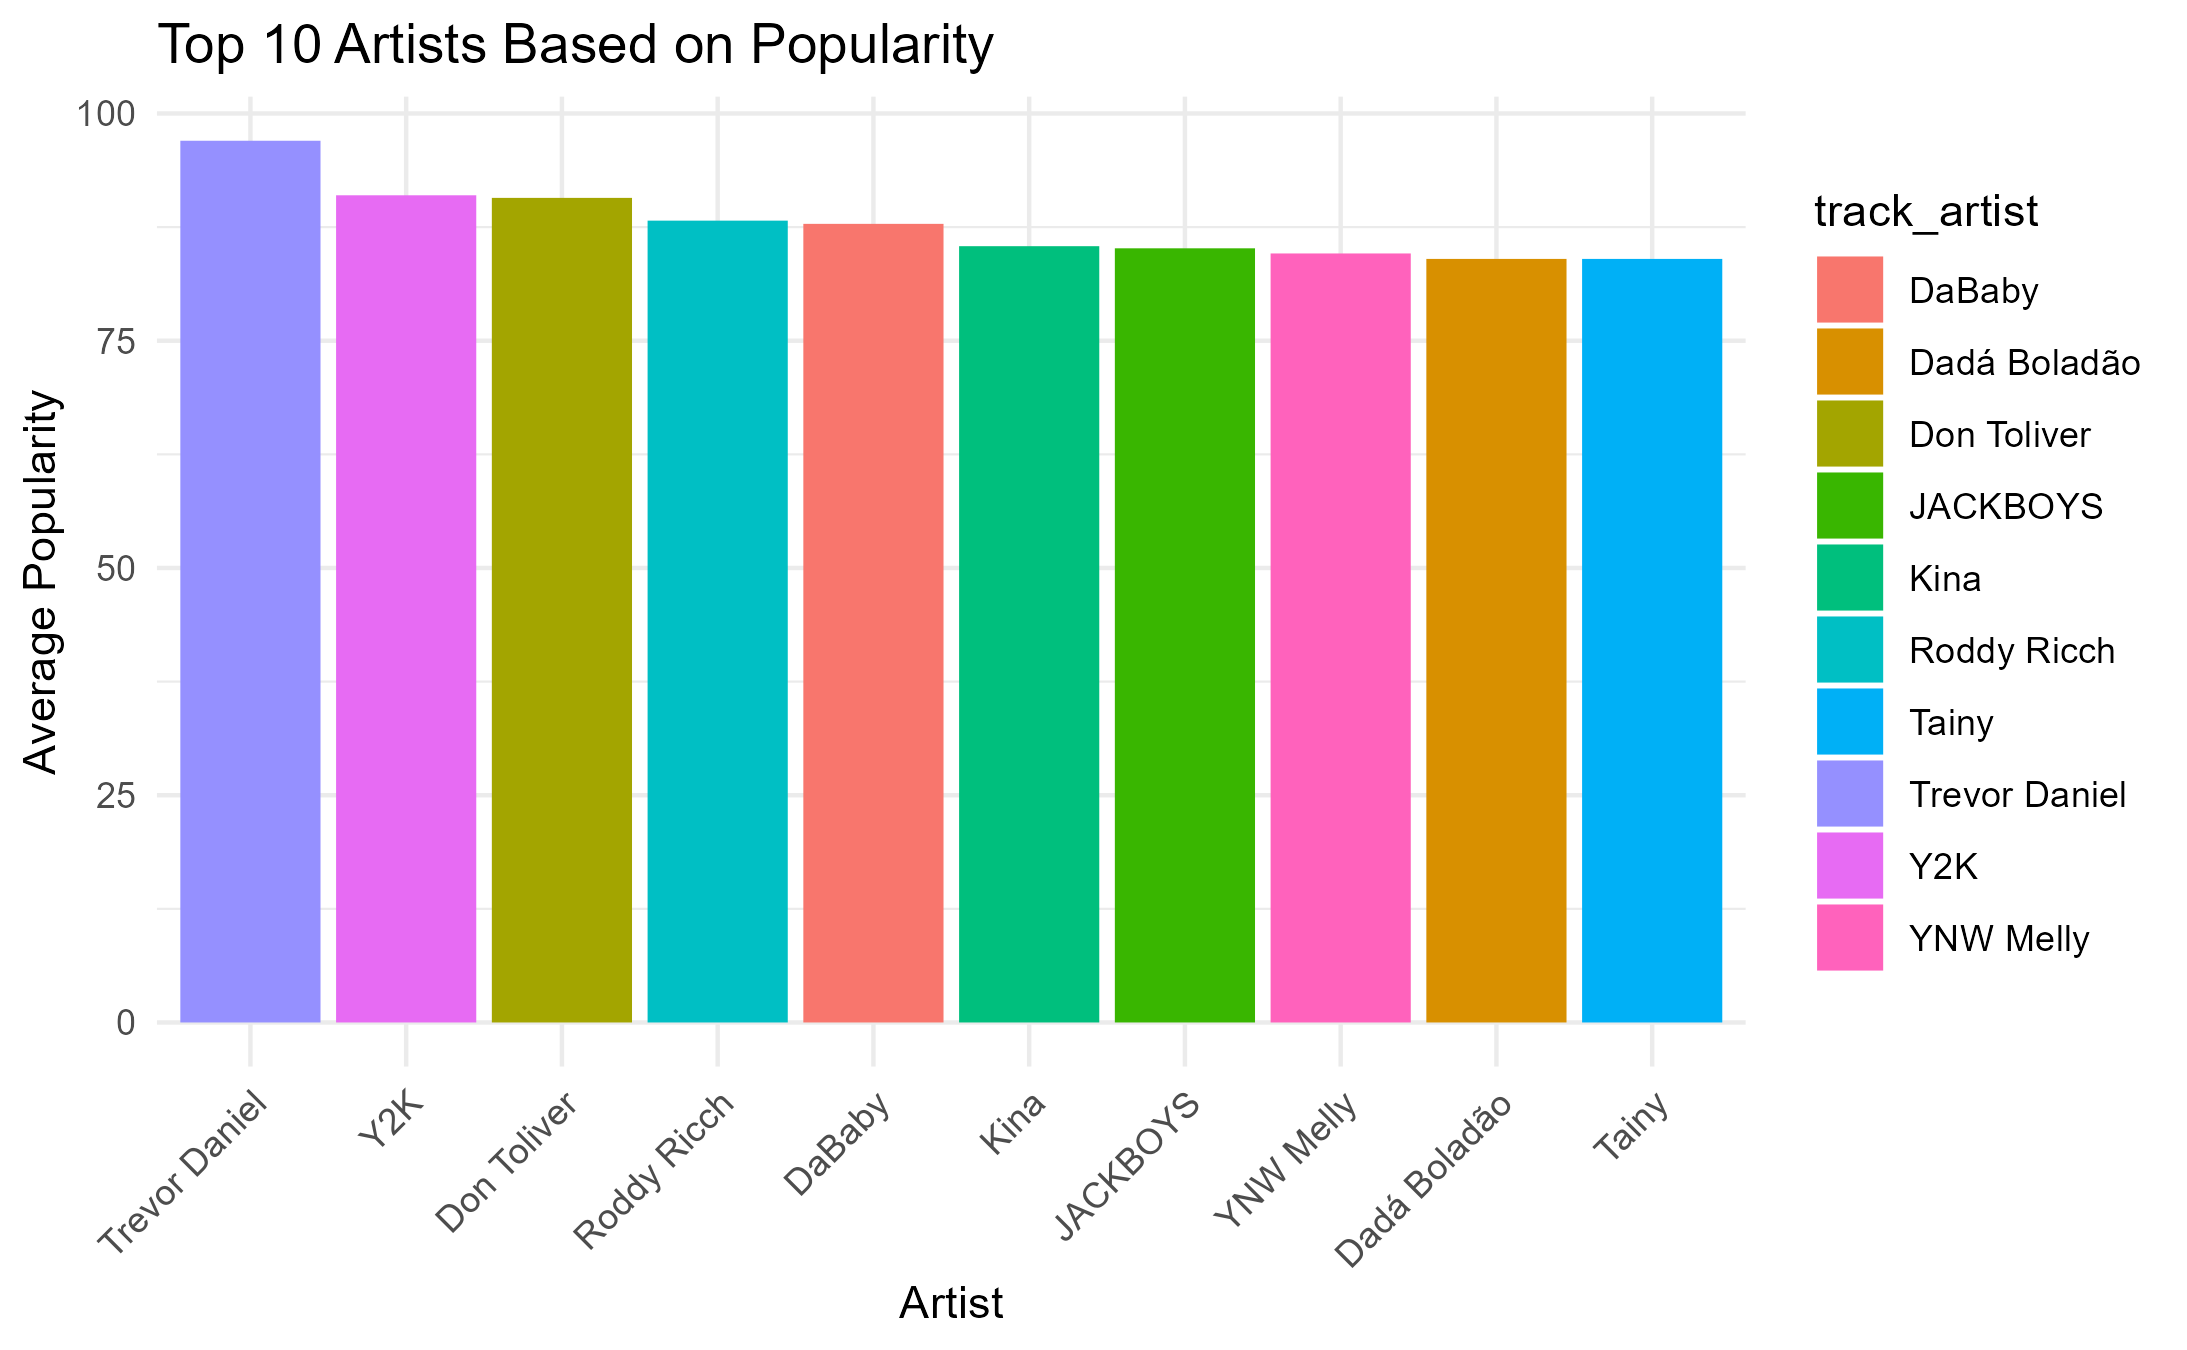
\includegraphics[scale=0.9]{slike/Top 10 popularity}
		%veličina slike u odnosu na originalnu datoteku i pozicija slike
		\centering
		\caption{Top 10 Artists Based on Popularity}
		
	\end{figure}





\section{Vizualizacija Podataka}
	Vizualizacija podataka postaje ključna komponenta analize i interpretacije kompleksnih skupova podataka. 
	U ovom podpoglavlju istražujemo moć vizualizacije u kontekstu glazbene platforme Spotify, prezentirajući neke od grafova kako bismo bolje razumjeli glazbene obrasce, preferencije slušatelja te dinamiku glazbene industrije.
	
	\subsubsection{1) Histogram of song popularity}
	
	\textbf{Opis grafa:}
	
	Ovaj graf prikazuje histogram popularnosti. Prikazuje distribuciju popularnosti pjesama. Na x-osi nalaze se razine popularnosti pjesama, a y-osi broj pjesama koje se nalaze u pojedinoj razini popularnosti.
	Ovaj histogram omogućava vizualni pregled koje su razine popularnosti češće, a koje rjeđe. 

	\textbf{Slika grafa:}
	\begin{figure}[H]
		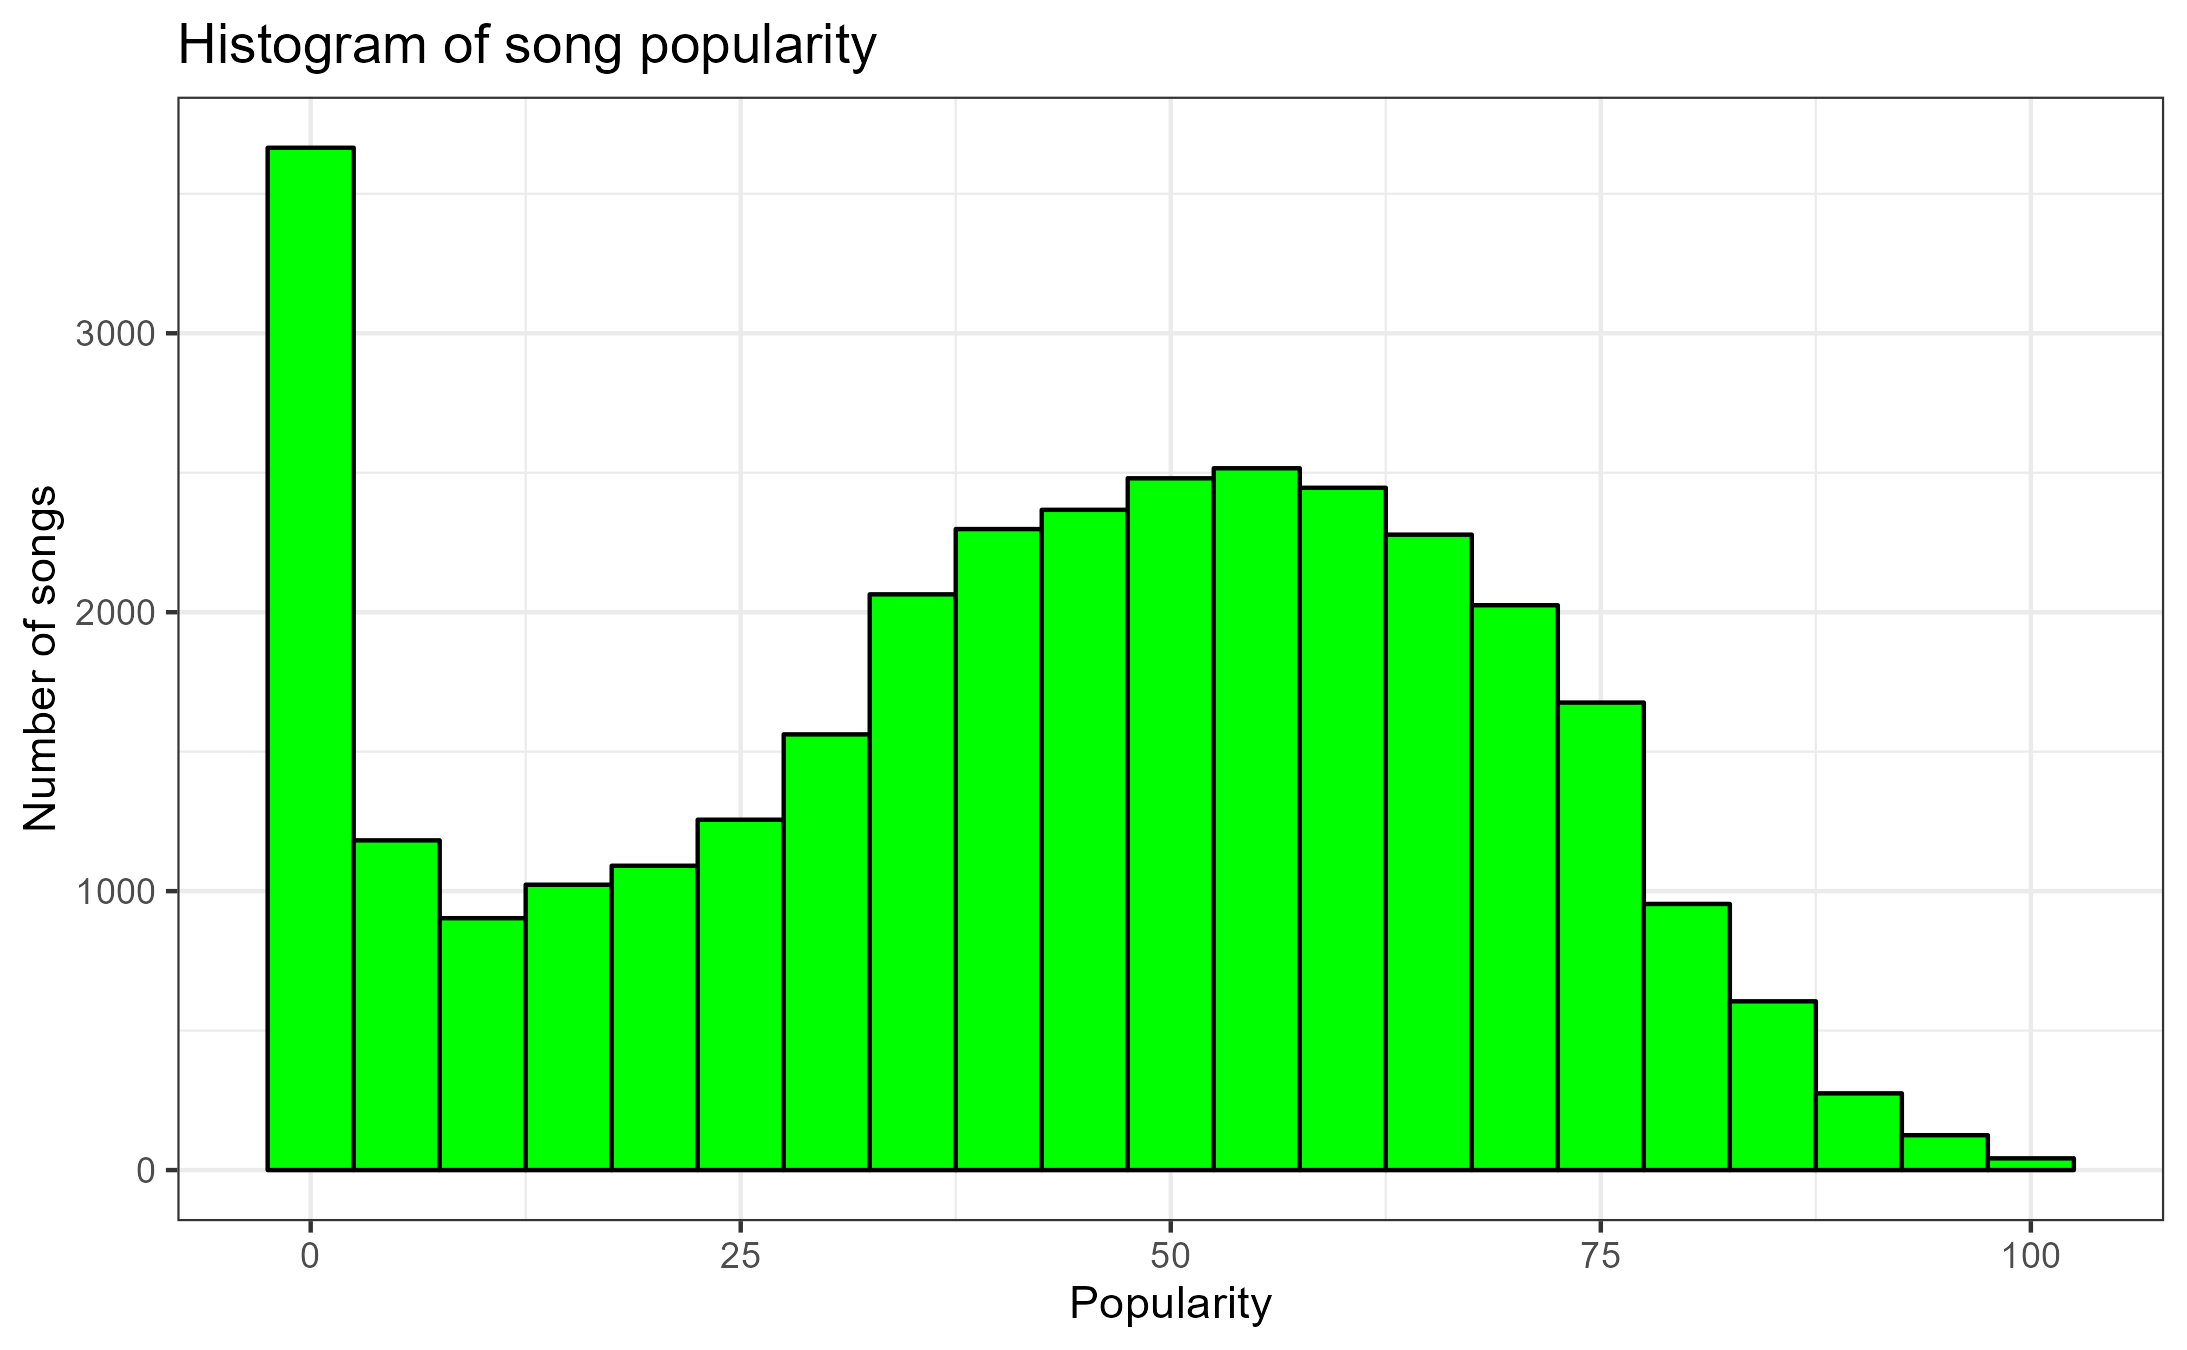
\includegraphics[scale=0.9]{slike/Histogram of song popularity.png}
		%veličina slike u odnosu na originalnu datoteku i pozicija slike
		\centering
		\caption{Histogram of song popularity}
		
	\end{figure}

	\subsubsection{2) Top 10 Artists Based on Popularity}
	
	\textbf{Opis grafa:}
	
	Ovaj graf prikazuje deset najpopularnijih glazbenih izvođača temeljem prosječne popularnosti njihovih pjesama. Izračunata je srednja vrijednost popularnosti za svakog izvođača, a zatim su odabrani najbolji deset izvođača prema toj mjeri popularnosti.
	
	Na x-osi su navedeni izvođači, poredani prema visini prosječne popularnosti, dok y-os prikazuje prosječnu popularnost. Svaki šareni stupac predstavlja jednog izvođača, a visina stupa označava njegovu prosječnu popularnost.
	
	Ovaj graf pruža brz i pregledan način usporedbe popularnosti izvođača, omogućujući identifikaciju najboljih deset temeljem prosjeka popularnosti njihovih pjesama.
	
	\textbf{Slika grafa:}
	\begin{figure}[H]
		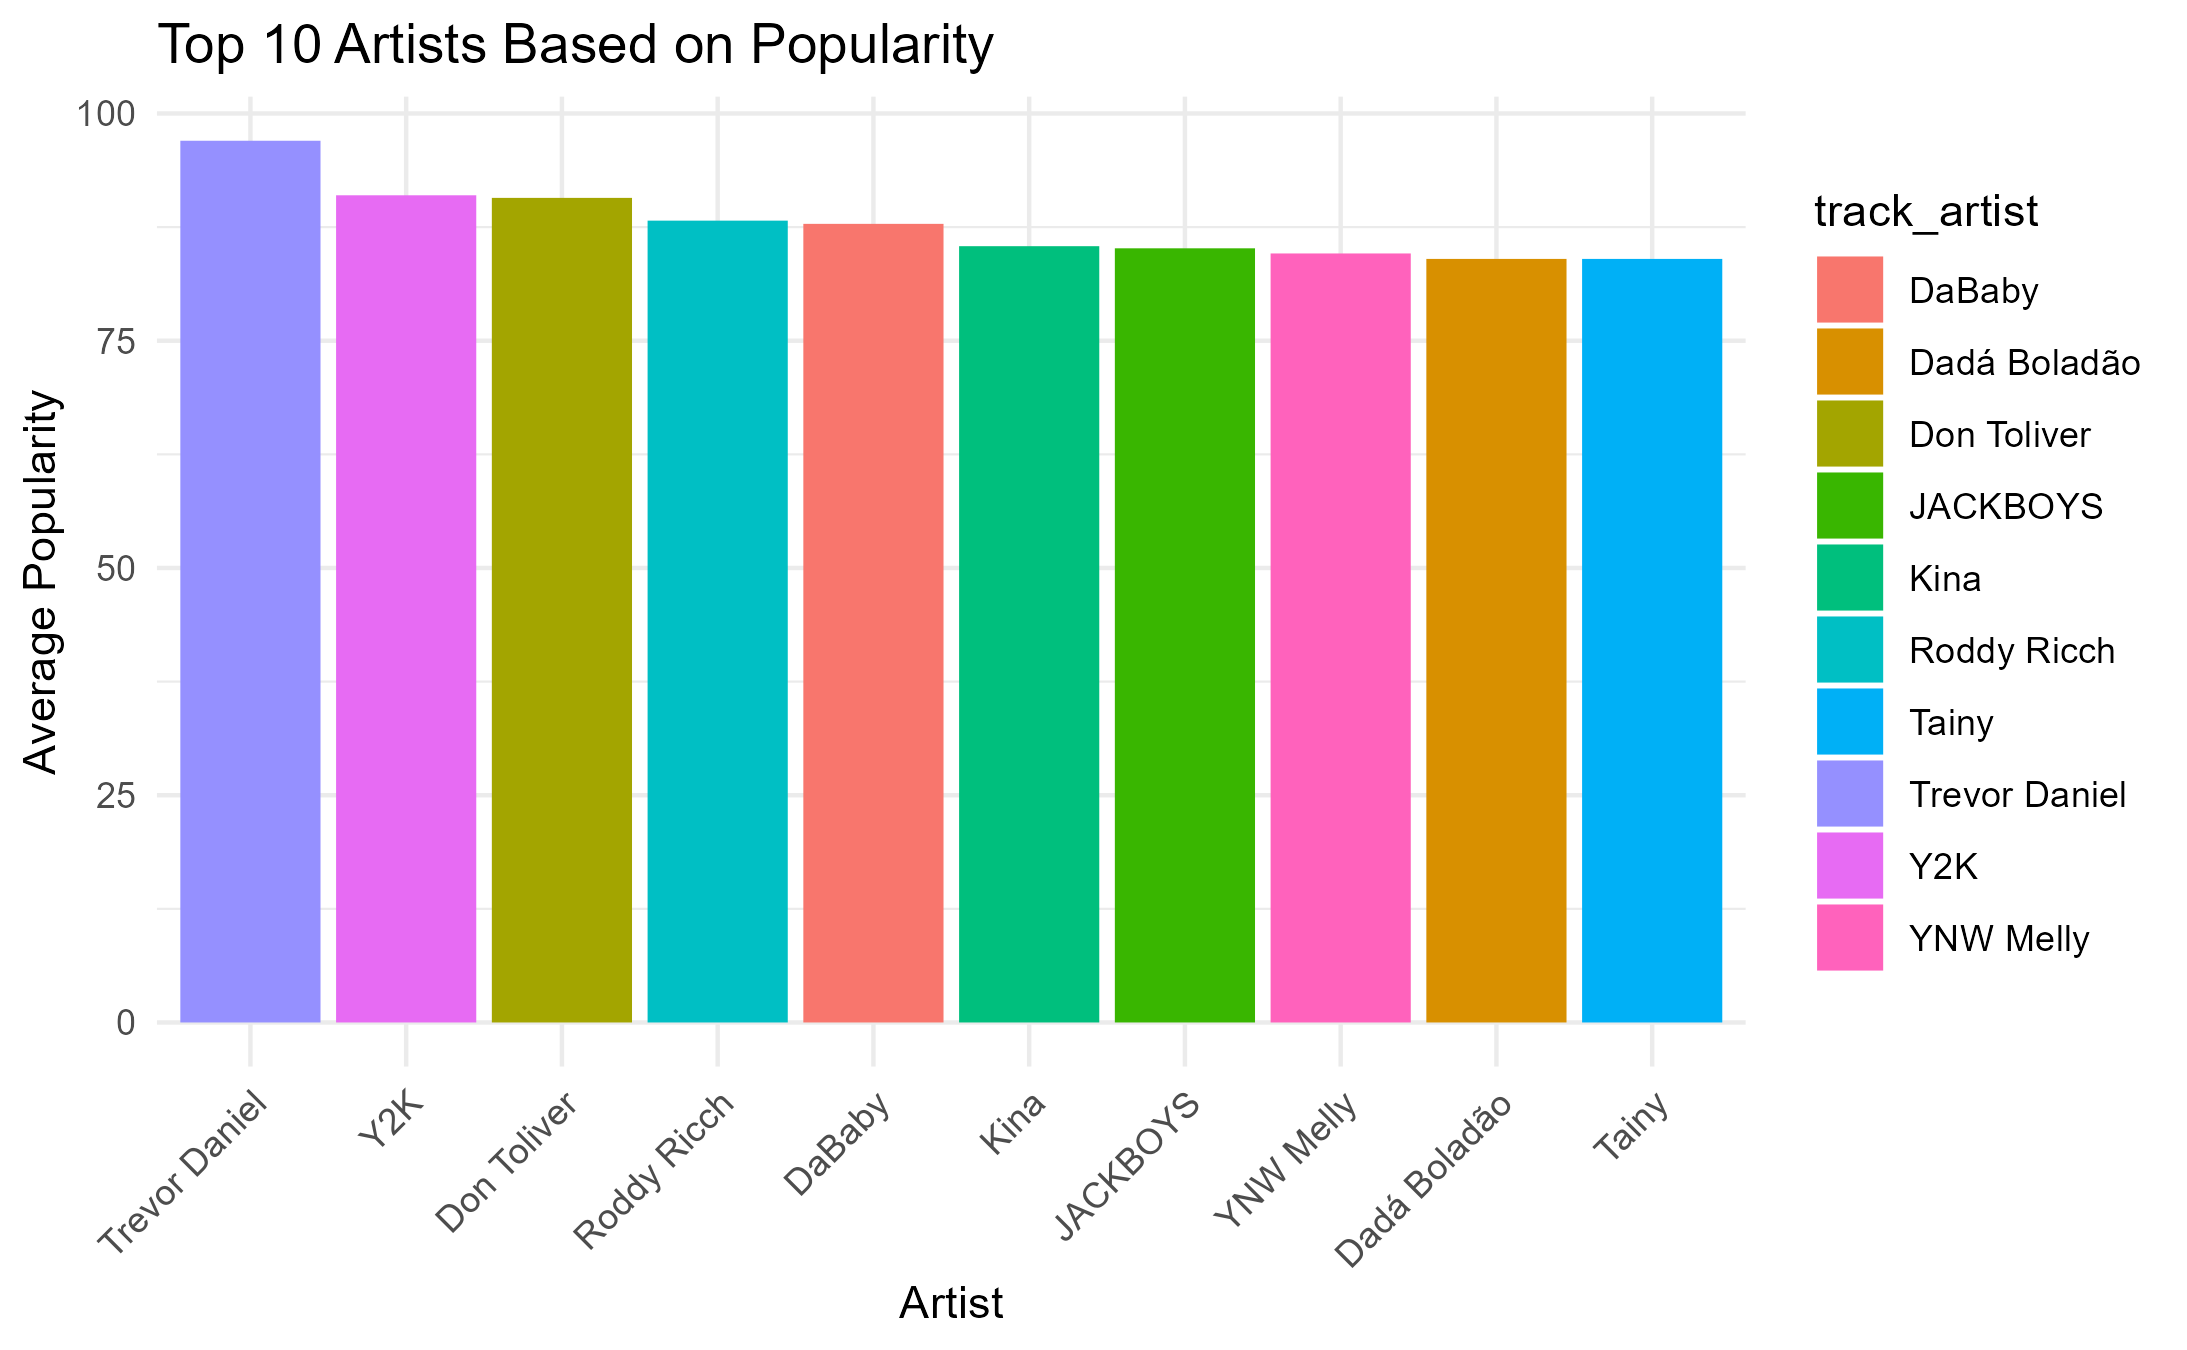
\includegraphics[scale=0.9]{slike/Top 10 popularity}
		%veličina slike u odnosu na originalnu datoteku i pozicija slike
		\centering
		\caption{Top 10 Artists Based on Popularity}
		
	\end{figure}


	\subsubsection{3) Average popularity of songs per year}
	
	\textbf{Opis grafa:}
	
	Ovaj stupčasti graf prikazuje prosječnu popularnost pjesama po godinama u razdoblju od 2000. godine do 2020. godine. X-os ovog grafa su godine u navedenom razdoblju (svaki stupac predstavlja jednu godinu), dok y-os predstavlja prosječnu popularnost. 
	Uvidom u ovaj graf možemo jednostavno vidjeti u kojoj su godini pjesme imale najveću popularnost, te vidjeti kako se popularnost mijenjala tokom tih 20 godina.

	
	\textbf{Slika grafa:}
	\begin{figure}[H]
		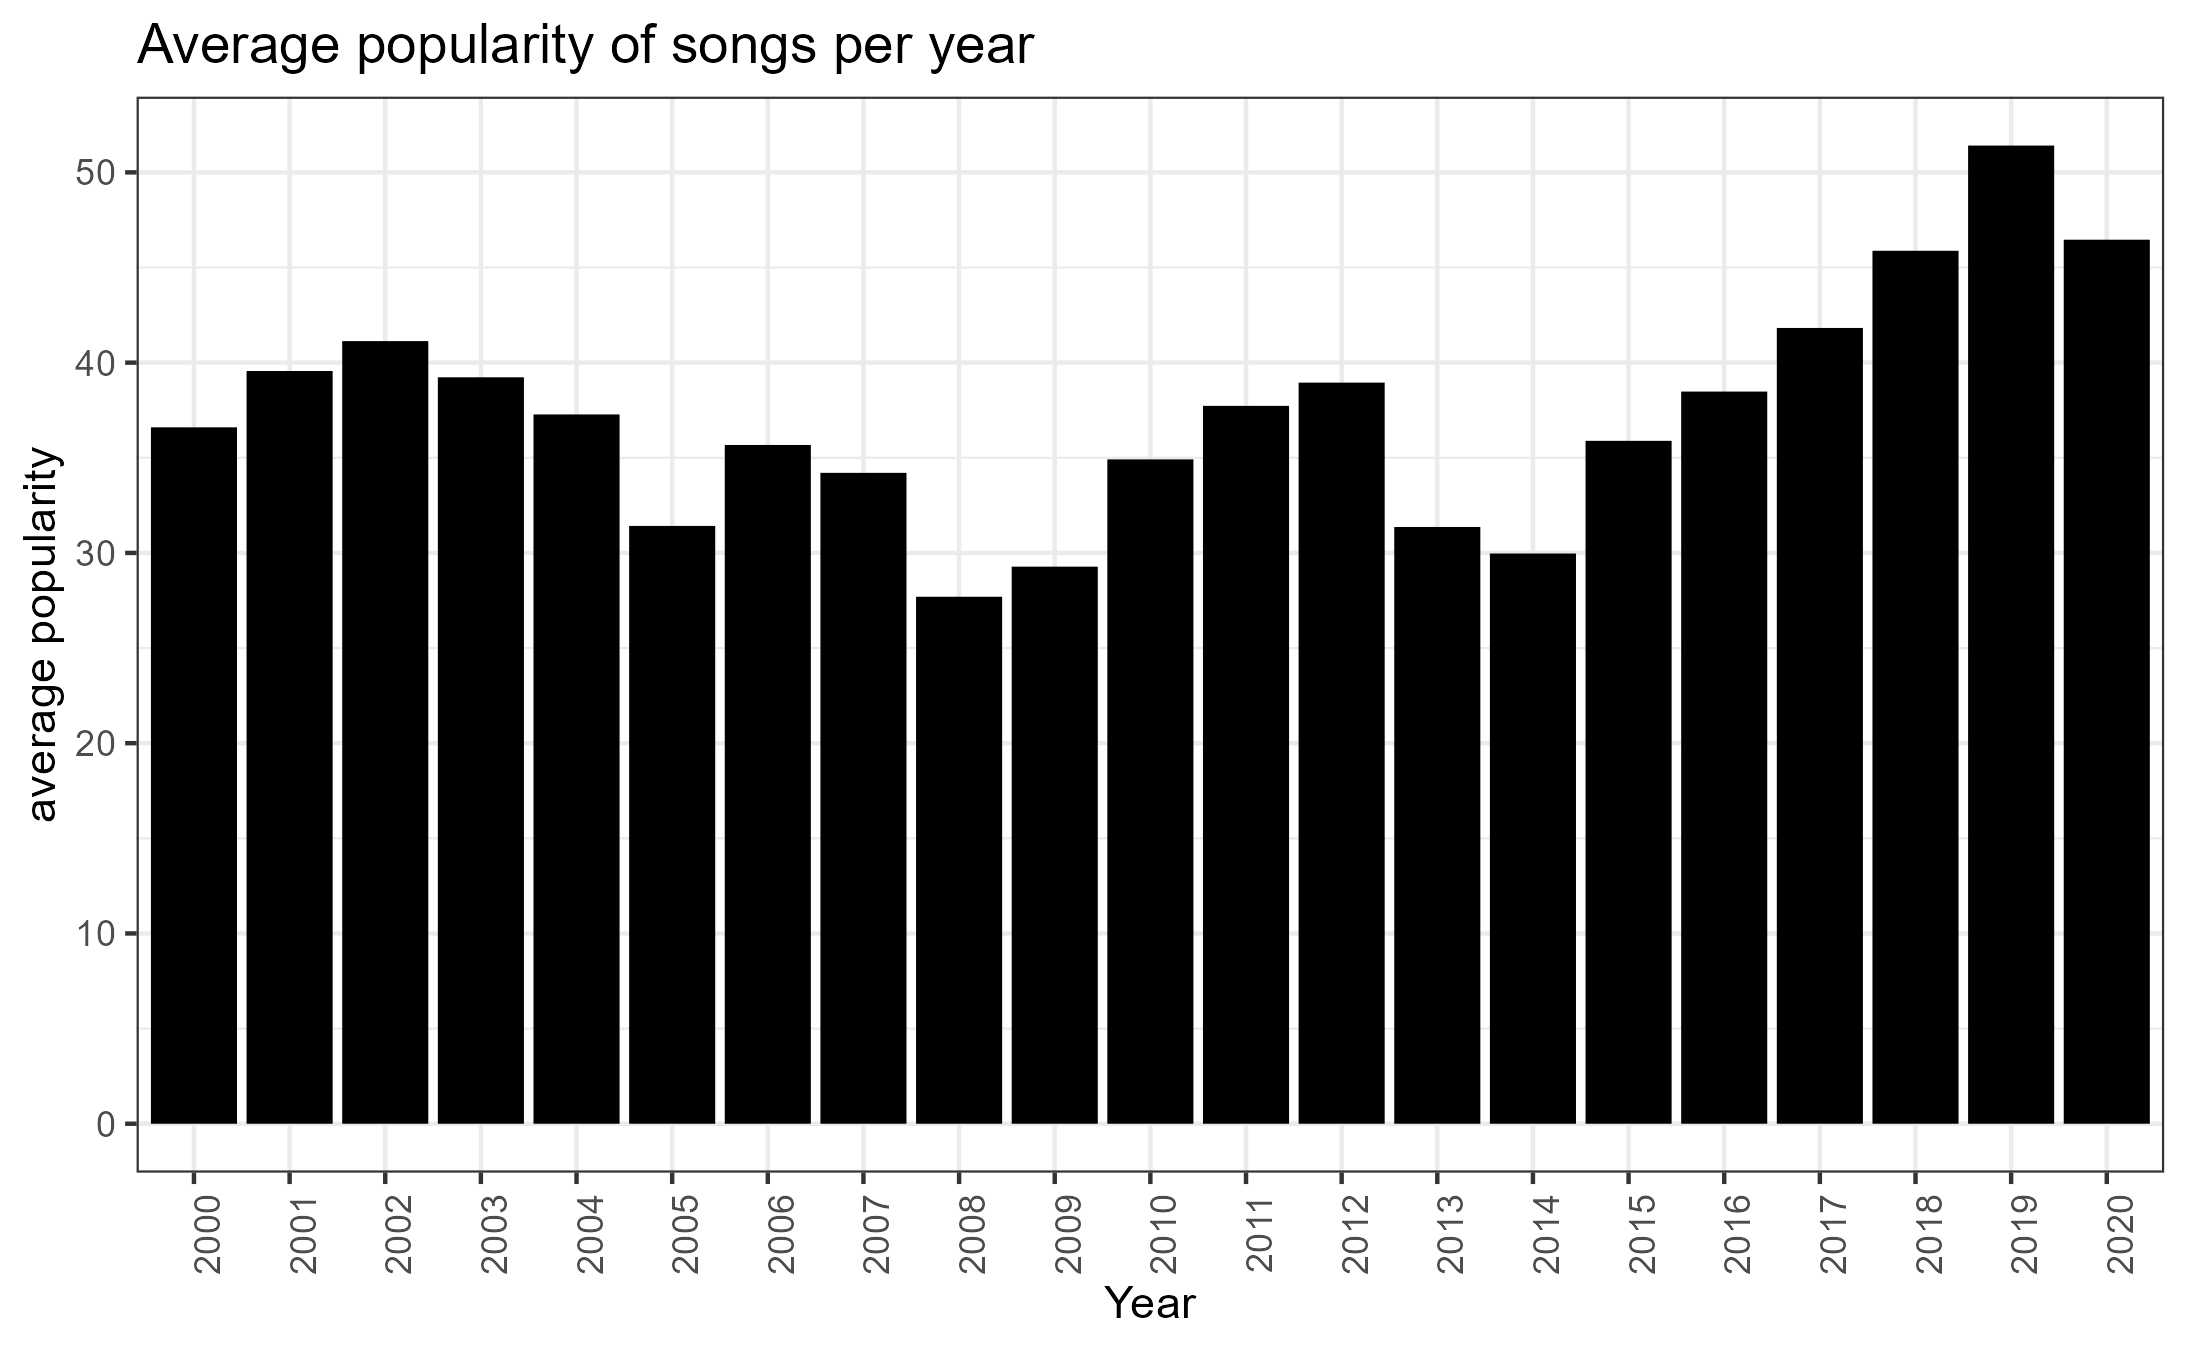
\includegraphics[scale=0.9]{slike/Average popularity of songs per year.png}
		%veličina slike u odnosu na originalnu datoteku i pozicija slike
		\centering
		\caption{Average popularity of songs per year}
		
	\end{figure}
	
		\subsubsection{4) Energy Distribution Across Playlist Genre}
	
	\textbf{Opis grafa:}
	
	Ovaj graf prikazuje distribuciju energije (y-os) na temelju različitih žanrova playlista (x-os). Svaki boxplot predstavlja jedan žanr, a njegova visina odražava raspon energije unutar tog žanra. Unutar svakog boxplota nalazi se pravokutnik koji predstavlja interkvartilni raspon, a linija unutar pravokutnika označava medijan energije.
	
	Dodatno, postojanje "notcha" u sredini svakog boxplota pruža informaciju o razlikama u medijanima između žanrova.
	
	
	\textbf{Slika grafa:}
	\begin{figure}[H]
		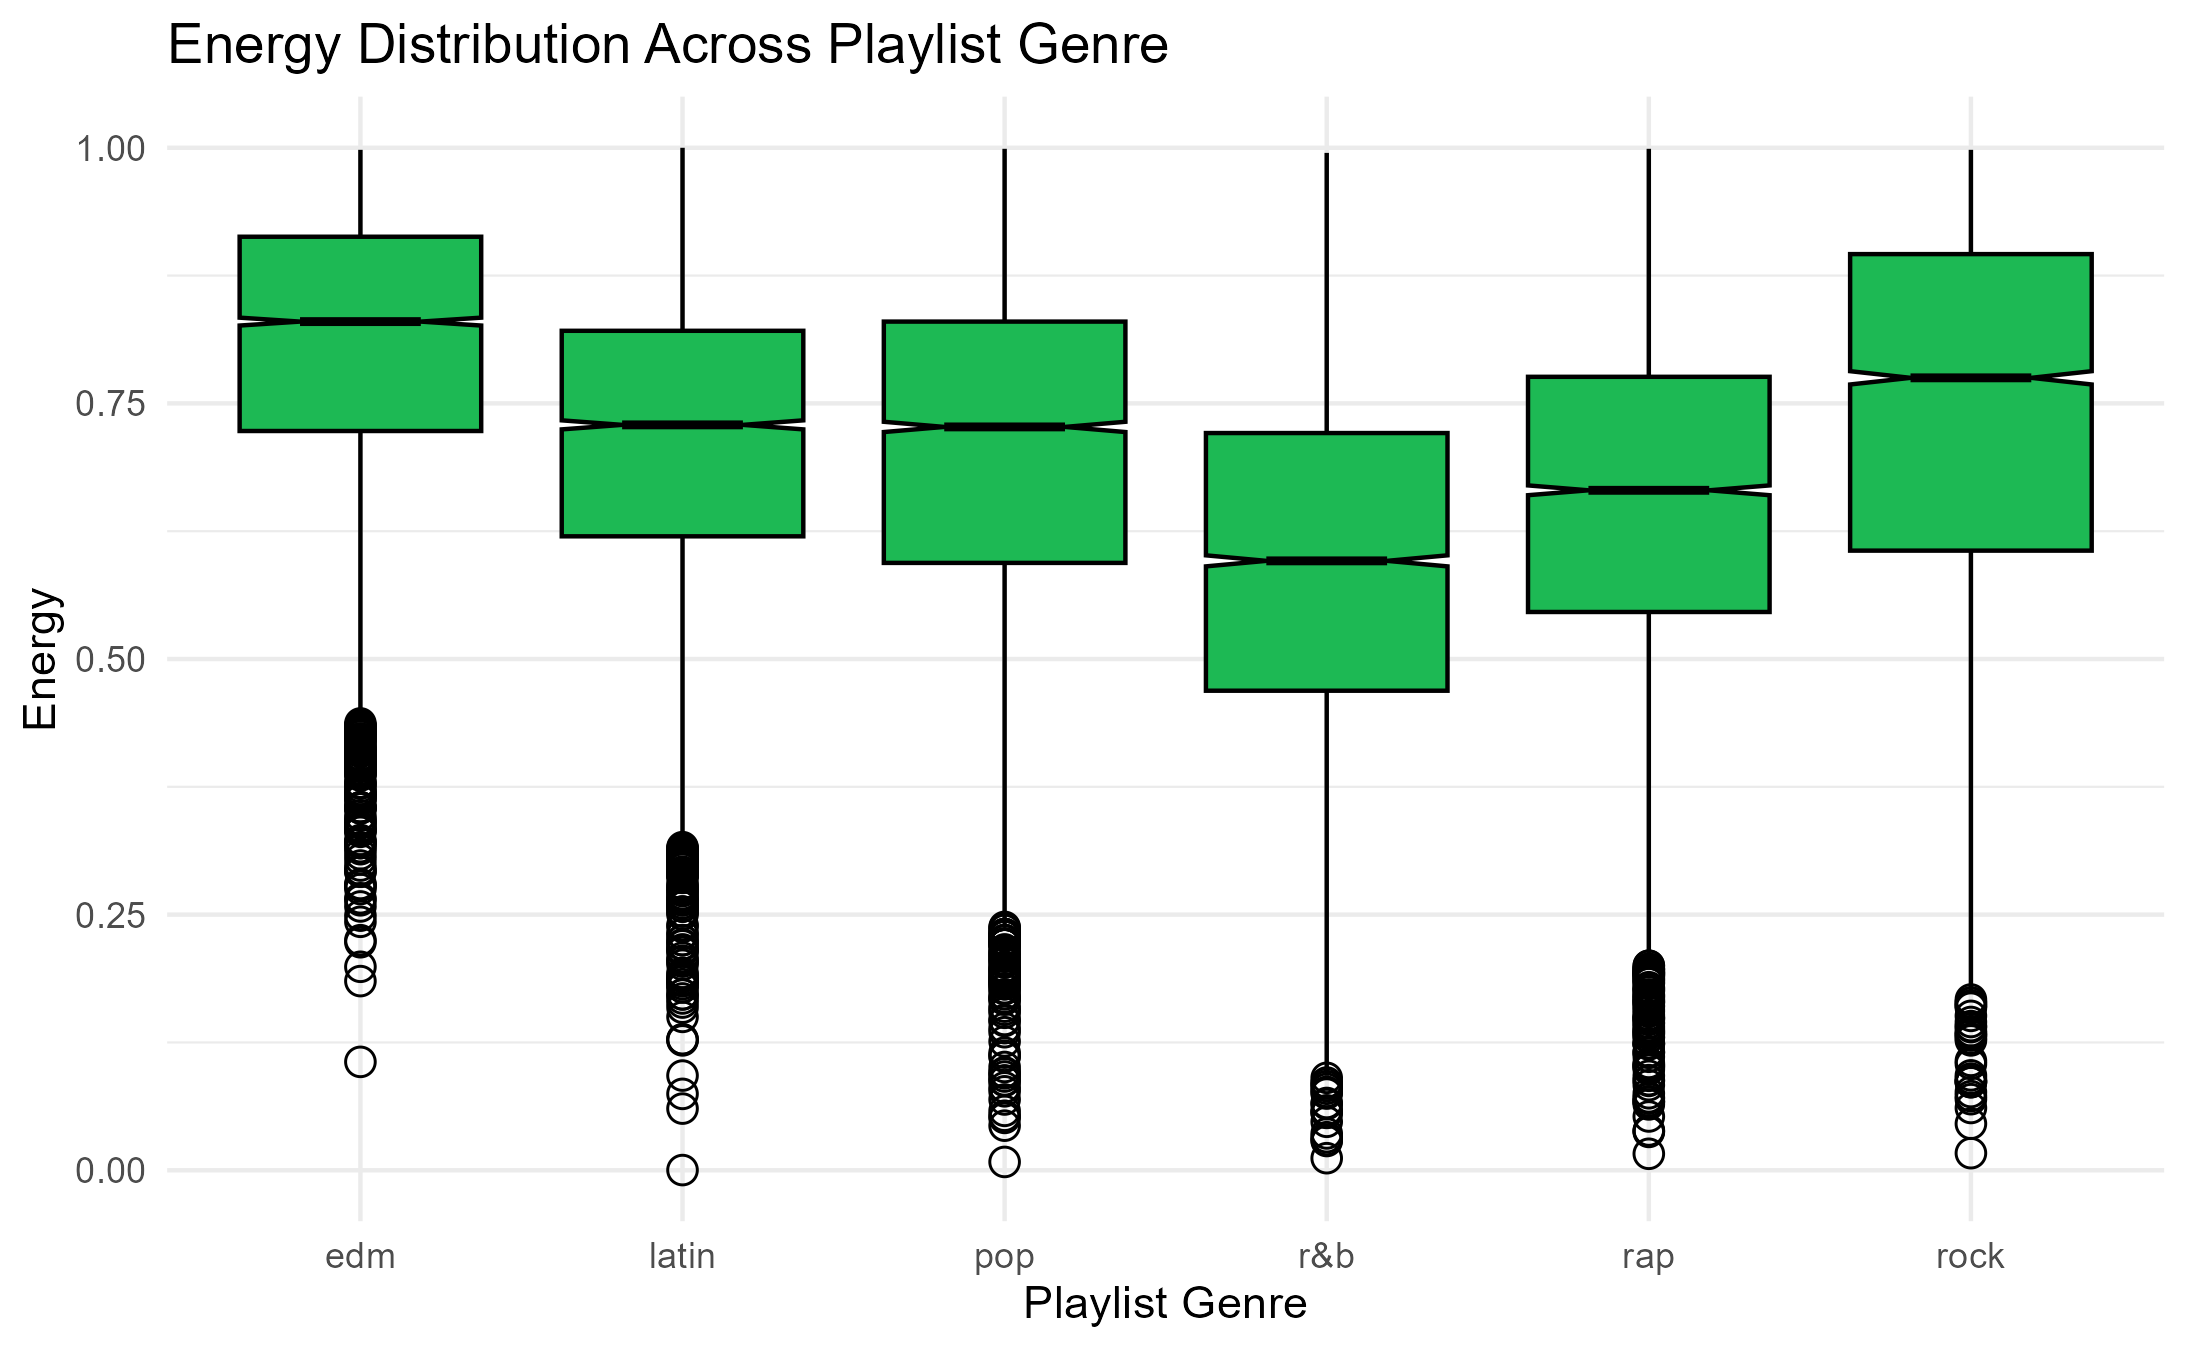
\includegraphics[scale=0.9]{slike/Genre-Energy.png}
		%veličina slike u odnosu na originalnu datoteku i pozicija slike
		\centering
		\caption{Energy Distribution Across Playlist Genre}
		
	\end{figure}
	
		\subsubsection{5) Distribution of Genres and Subgenres}
	
	\textbf{Opis grafa:}
	
		Ovaj graf prikazuje broj playlista unutar određenih glavnih žanrova, razdijeljenih prema podžanrovima. Na x-osi su navedeni glavni žanrovi playlista, dok y-os pokazuje broj playlista. Svaki šareni segment na stupcu predstavlja određeni podžanr unutar glavnog žanra.
		
		Stupci su složeni jedan na drugi kako bi se vizualno prikazala distribucija podžanrova u okviru svakog glavnog žanra. 
	
	
	\textbf{Slika grafa:}
	\begin{figure}[H]
		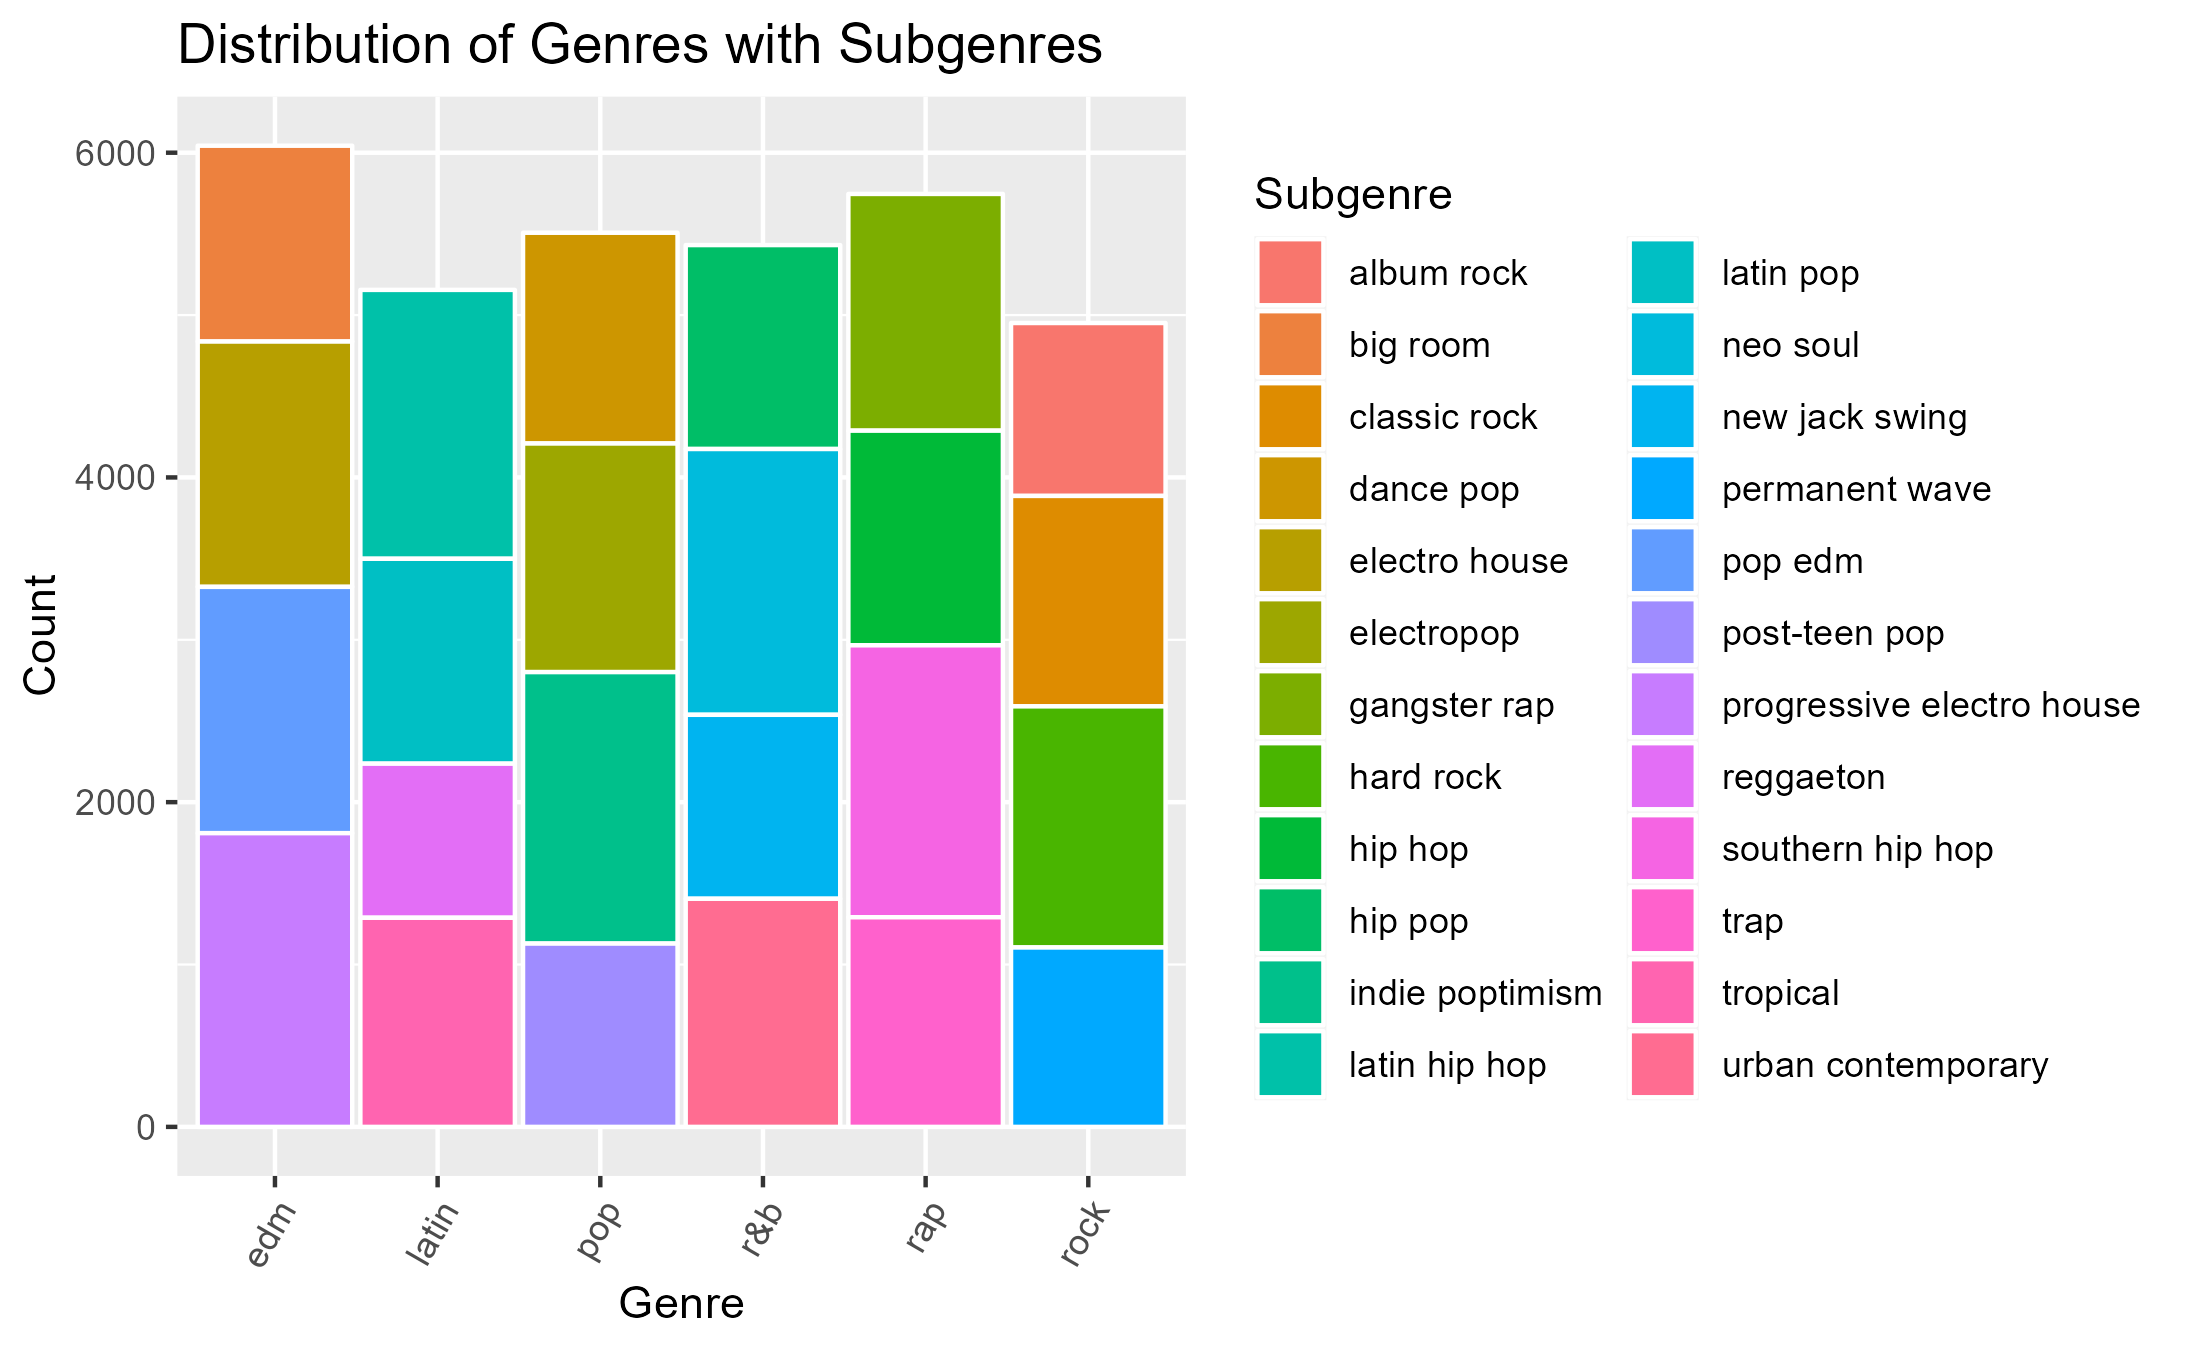
\includegraphics[scale=0.9]{slike/Genre-Subgenre.png}
		%veličina slike u odnosu na originalnu datoteku i pozicija slike
		\centering
		\caption{Distribution of Genres and Subgenres}
		
	\end{figure}
	
		\subsubsection{6) Danceability and Energy with Popularity}
	
	\textbf{Opis grafa:}
	
	Ovaj šareni graf prikazuje odnos između plesnosti (x-os) i energije (y-os) za različite glazbene pjesme. Svaka točka na grafu predstavlja pojedinu pjesmu, a njezina boja označava razinu popularnosti. Tamnije crvene nijanse označavaju popularnije pjesme, dok svjetlije plave nijanse ukazuju na manju popularnost.
	
	Graf pruža uvid u raznolikost glazbenih preferencija te naglašava da glazbene osobitosti kao što su plesnost i energija nisu nužno ključni faktori koji određuju popularnost pjesama na temelju analize ovog skupa podataka.
	
	\textbf{Slika grafa:}
	\begin{figure}[H]
		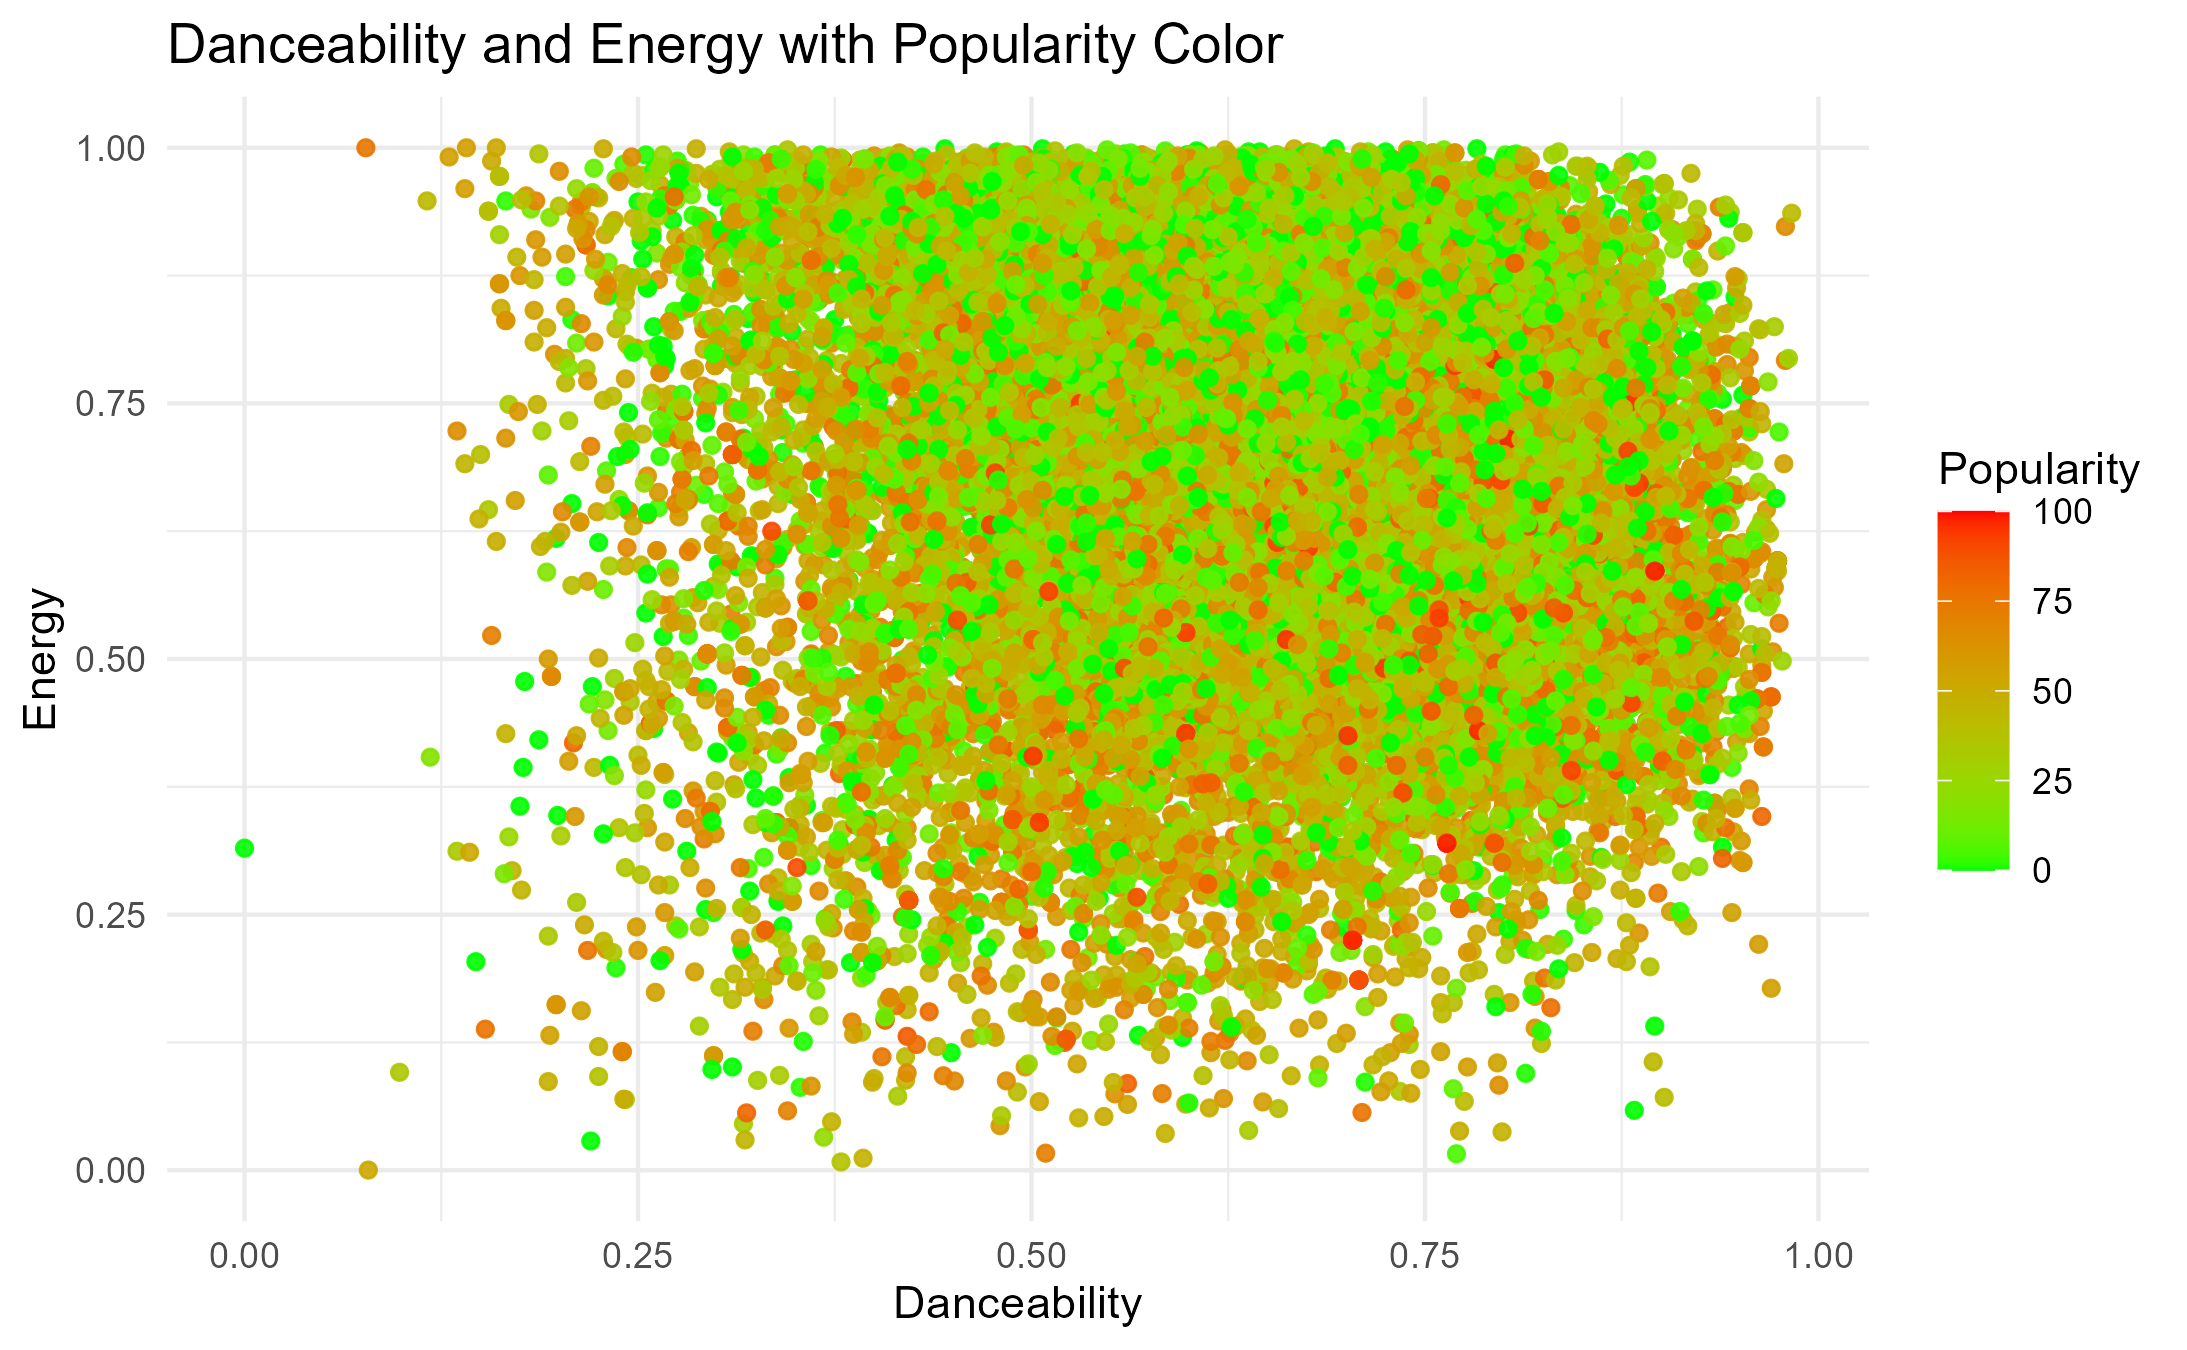
\includegraphics[scale=0.9]{slike/Dance-Energy-popularity.png}
		%veličina slike u odnosu na originalnu datoteku i pozicija slike
		\centering
		\caption{ Danceability and Energy with Popularity}
		
	\end{figure}


\eject



